% ==================================================================
% APPENDIX A5 — ISW amplitude: extraction of ε (PROVISIONAL proxy).
%
% FINAL DRAFT on freeze-checkpoint numbers (2026-04-19).
% Numerics: scripts/epsilon_convergence/ch3_isw.py, result_ch3.json
% Background: scripts/epsilon_convergence/ect_background.py
%         (USED for bookkeeping consistency only; kernel κ_ISW
%          NOT recalibrated on ECT-native background)
%
% Structure (unified per-probe template shared with A1-A4):
%   A5.1  Physics of the probe
%   A5.2  Observational inputs
%   A5.3  ECT-side model and extraction scope
%         (WITH EXPLICIT PROVISIONAL LABELLING per GPT r21)
%   A5.4  Extraction statistic
%   A5.5  Interval definition and origin of the width
%   A5.6  Figure
%   A5.7  Methodological limitations
%
% Character of this channel (GPT r21 requirement of maximum honesty):
%   Proxy-level only.
%   Kernel NOT recalibrated on common background.
%   Kept as provisional consistency channel.
%   NOT at the same epistemic level as A1/A2/A3/A4.
%   Must be stated up front and repeatedly.
%
% NO integration into preprint yet.
% ==================================================================

\section{Extraction of the effective uniform-$\varepsilon$ interval
from the ISW channel (provisional proxy)}
\label{app:eps_extraction_isw}

This appendix derives the effective uniform-$\varepsilon$ upper
bound from the late-time Integrated Sachs-Wolfe (ISW) amplitude.
The present extraction is deliberately presented as a
\emph{provisional proxy}, not as an extraction at the same
epistemic level as A1--A4. The reasons are stated up front and in
each subsection:
\begin{itemize}
  \item the $\varepsilon$-dependence of the observable is
        linearised,
  \item the proportionality coefficient $\kappa_{\rm ISW}$ is
        calibrated against a $\Lambda$CDM-background Limber
        weight function and has \emph{not} been recalibrated
        against the common ECT background of
        Appendix~\ref{app:eps_methodology} in the present
        freeze checkpoint,
  \item the observational uncertainty is very large (of order
        $30\%$) and the channel cannot by itself extract a
        non-trivial central value.
\end{itemize}
The retained result of this channel is therefore a broad
one-sided upper bound under the physical prior
$\varepsilon \geq 0$, whose numerical value is unchanged between
the pre-recalc and the post-recalc retained-pipeline and whose
interpretation is consistency-checking rather than evidential.

\subsection*{A5.1\quad Physics of the probe}

The late-time ISW effect is the cross-correlation between the
CMB temperature anisotropy and tracers of the large-scale
gravitational potential $\Phi$ at low redshift. In a matter-only
universe the gravitational potential is constant in time on large
scales, and the ISW signal vanishes; the presence of dark
energy causes $\dot\Phi \neq 0$ at low $z$, which gives a
non-zero cross-correlation. In the effective uniform-$\varepsilon$
layer of \S\ref{subsec:eps_def_rebuilt}, the deformation of the
expansion rate through \eqref{eq:eps_friedmann_A1} modifies the
late-time decay of $\Phi$, and the amplitude of the resulting
ISW signal deviates from its $\Lambda$CDM value.

\subsection*{A5.2\quad Observational inputs}

The observable is the measured amplitude of the cross-correlation
between the Planck CMB temperature map and the unWISE galaxy
catalogue, parametrised as a rescaling of the $\Lambda$CDM
prediction:
\begin{equation}
A_{\rm ISW}^{\rm obs} \;=\; 0.96 \pm 0.30,
\end{equation}
from Krolewski et al.\ 2024 \cite{Krolewski2024}. The central
value is $1\sigma$ below the $\Lambda$CDM-based prediction
$A_{\rm ISW}^{\Lambda} = 1$; the uncertainty of $30\%$ is
intrinsically large, and the measurement cannot be sharpened
within the present pipeline.

\subsection*{A5.3\quad ECT-side model and extraction scope
(provisional)}

At the provisional-proxy level used here, the
$\varepsilon$-dependence of the ISW amplitude is approximated by
the linearised form
\begin{equation}
A_{\rm ISW}^{\rm model}(\varepsilon)
\;=\;
1 + \kappa_{\rm ISW}\,\varepsilon,
\qquad
\kappa_{\rm ISW} \;\approx\; 6,
\label{eq:A_ISW_model}
\end{equation}
where the coefficient $\kappa_{\rm ISW}$ was obtained from a
single-zoomed Limber integration of the ISW weight function under
a $\Lambda$CDM background. This coefficient has \emph{not} been
recalibrated against the common ECT background of
Appendix~\ref{app:eps_methodology} in the present checkpoint.
The justification for this deferral is stated in the
freeze-checkpoint methodology (A6): a genuine ECT-background
recalibration of $\kappa_{\rm ISW}$ would require re-integrating
the full late-time ISW weight function $W_{\rm ISW}(z)$ under
$H(z, \varepsilon)$, $t(z, \varepsilon)$, and $\dot\Phi(z, \varepsilon)$
trajectories, which is beyond the scope of Phase 2A.

\paragraph{Held fixed under the present proxy.}
The linearised form \eqref{eq:A_ISW_model}; the
$\Lambda$CDM-background-calibrated coefficient
$\kappa_{\rm ISW} = 6$; the Krolewski+2024 observational anchor.

\paragraph{Varied.}
$\varepsilon$ only.

\paragraph{Not included at this proxy level.}
Any nonlinear dependence of $A_{\rm ISW}$ on $\varepsilon$;
recalibration of $\kappa_{\rm ISW}$ on the common ECT background;
cross-correlations with other late-time probes (weak lensing,
$f\sigma_8$) that would share systematic effects; full Boltzmann
evolution of $\dot\Phi$ under the ECT deformation.

\subsection*{A5.4\quad Extraction statistic}

The one-parameter model gives the inversion
\begin{equation}
\varepsilon(A_{\rm ISW})
\;=\;
\frac{A_{\rm ISW} - 1}{\kappa_{\rm ISW}}.
\end{equation}
The raw best-fit and the raw $1\sigma$ and $2\sigma$ intervals
follow from the $\pm 1\sigma$ and $\pm 2\sigma$ observational
brackets on $A_{\rm ISW}^{\rm obs}$.

\subsection*{A5.5\quad Interval definition and origin of the width}

\paragraph{Raw result.}
Direct inversion of $A_{\rm ISW}^{\rm obs} = 0.96 \pm 0.30$ gives
\begin{align}
\varepsilon_{\rm raw}
&\;=\; -0.0067,
\\[2pt]
[\varepsilon_{\rm lo}^{1\sigma},\,\varepsilon_{\rm hi}^{1\sigma}]_{\rm raw}
&\;=\; [\,-0.057,\ +0.043\,],
\\[2pt]
[\varepsilon_{\rm lo}^{2\sigma},\,\varepsilon_{\rm hi}^{2\sigma}]_{\rm raw}
&\;=\; [\,-0.107,\ +0.093\,].
\end{align}
The raw best-fit is indistinguishable from zero within the
observational uncertainty.

\paragraph{Retained interval under the physical prior.}
Imposing $\varepsilon \geq 0$, the ISW channel contributes a
one-sided upper bound:
\begin{align}
[\varepsilon_{\rm lo}^{1\sigma},\,\varepsilon_{\rm hi}^{1\sigma}]
&\;=\;
[\,0,\ 0.0433\,],
\\[2pt]
[\varepsilon_{\rm lo}^{2\sigma},\,\varepsilon_{\rm hi}^{2\sigma}]
&\;=\;
[\,0,\ 0.0933\,].
\end{align}
The interval was numerically unchanged between the pre-recalc and
the post-recalc retained pipelines, reflecting the fact that
$\kappa_{\rm ISW}$ has not yet been recalibrated.

\paragraph{Origin of the width.}
The $\pm 30\%$ observational uncertainty on $A_{\rm ISW}^{\rm obs}$
is the sole driver of the width. There is no fitting at all: the
channel is a direct algebraic inversion of a linearised
one-parameter model, and the reported interval simply reflects
the observational bracket on $A_{\rm ISW}$ through
\eqref{eq:A_ISW_model}.

\paragraph{Channel character.}
The ISW channel is a consistency channel only. Its retained upper
bound is broader than those of A1--A4 and does not bind the joint
interval. Its principal role in
\S\ref{subsec:eps_retained_rebuilt} is to demonstrate that the
retained joint band $[0.0296,\,0.0376]$ is compatible with an
independent late-time observable, \emph{not} to contribute
evidential weight to the band.

\subsection*{A5.6\quad Figure}

\begin{figure}[H]
\centering
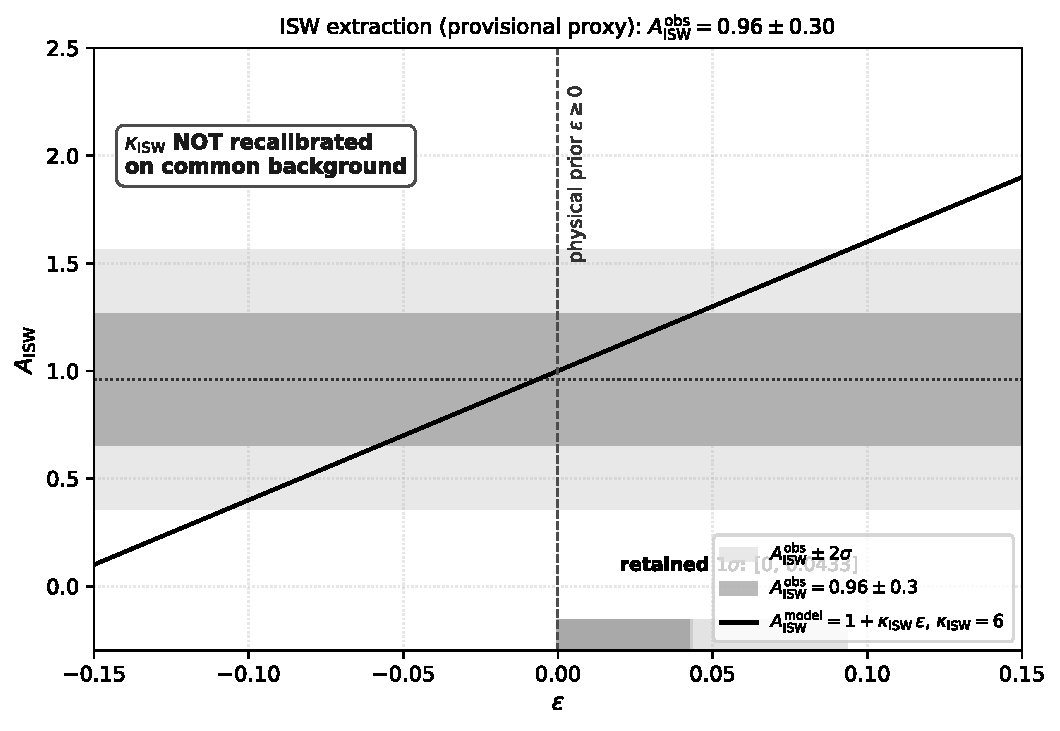
\includegraphics[width=0.82\textwidth]{figures/fig_isw_extraction_bw.pdf}
\caption{Extraction of the effective $\varepsilon$-upper bound
from the ISW channel, at the provisional proxy level described
in A5.3. The linearised model
$A_{\rm ISW}(\varepsilon) = 1 + \kappa_{\rm ISW}\varepsilon$ with
$\kappa_{\rm ISW} = 6$ (solid line) is compared with the
observational anchor $A_{\rm ISW}^{\rm obs} = 0.96 \pm 0.30$
(horizontal darker gray band: $1\sigma$; lighter: $2\sigma$). The
inverted $\varepsilon$-intervals (shown along the
$\varepsilon$-axis below) are clipped to the physical region
$\varepsilon \geq 0$, yielding the retained one-sided upper bounds
$[0,\,0.0433]$ ($1\sigma$) and $[0,\,0.0933]$ ($2\sigma$). The
text ``$\kappa_{\rm ISW}$ not recalibrated'' is placed on the
figure to reinforce the provisional status. All shading and line
styles are grayscale per preprint convention.}
\label{fig:isw_extraction}
\end{figure}

\subsection*{A5.7\quad Methodological limitations}

\textit{(i) Linearised $\varepsilon$-dependence.}
The form \eqref{eq:A_ISW_model} truncates the
$\varepsilon$-dependence at linear order. For
$|\varepsilon| \gtrsim 0.05$ the linear approximation begins to
break down, and a non-linear recalculation of
$A_{\rm ISW}(\varepsilon)$ would be required to make the
extracted bound quantitative at the retained-band level. Since the
retained $1\sigma$ upper $0.043$ is close to this boundary, the
bound should be read as an order-of-magnitude consistency check
rather than a precise constraint.

\textit{(ii) $\kappa_{\rm ISW}$ not recalibrated on common
background.}
The coefficient $\kappa_{\rm ISW} = 6$ was calibrated under
$\Lambda$CDM-background Limber weights. On the common ECT
background of Appendix~\ref{app:eps_methodology}, the late-time
ISW weight function $W_{\rm ISW}(z)$ is modified through both
$H(z, \varepsilon)$ (which changes the conformal-time kernel) and
$\dot\Phi(z, \varepsilon)$ (which changes the source amplitude).
A self-consistent recalculation would, in principle, shift
$\kappa_{\rm ISW}$ by an unknown amount; the present checkpoint
therefore treats the retained ISW interval as provisional, and
the numerical value quoted in
\S\ref{subsec:eps_retained_rebuilt} is inherited from the
$\Lambda$CDM-background calibration.

\textit{(iii) Large observational uncertainty.}
The $\pm 30\%$ uncertainty on $A_{\rm ISW}^{\rm obs}$ is
intrinsically large and cannot be reduced within the present
pipeline. Even a perfectly recalibrated $\kappa_{\rm ISW}$ would
not sharpen the retained interval below approximately
$[0,\,0.03]$ at $1\sigma$.

\textit{(iv) Epistemic status.}
The ISW channel is not at the same epistemic level as A1--A4. In
the retained-five-probe analysis it functions as a consistency
check only: it does not bind any edge of the joint band, and its
numerical value is unchanged between the pre-recalc and
post-recalc pipelines. Any future strengthening of the ISW bound
(e.g., through kernel recalibration on the common background or
through tighter $A_{\rm ISW}^{\rm obs}$ measurements) would
naturally be incorporated into a future iteration of the retained
pipeline.

% ==================================================================
% END Appendix (extraction, ISW channel, provisional proxy).
% ==================================================================
